{

\setlength{\parindent}{0pt}
\setlength{\parskip}{1em}

\section{Background}
\subsection{State-of-the-art CNNs for Cloud Image Segmentation}

CNNs are a class of neural networks that apply small, learnable filters --- known as convolutional kernels --– across an image to extract spatial features. A CNN typically consists of multiple convolutional layers stacked sequentionally. Each layer applies a set of filters that capture different visual patterns, such as edges or textures. As the network goes deeper, the spatial resolution of the image decreases, while the depth (i.e., number of channels) increases. This is a result of applying multiple filters and optionally using pooling layers, which downsample feature maps to reduce computational complexity and introduce spatial invariance.

In image segmentation tasks such as cloud detection, preserving spatial resolution is critical. Therefore, architectures often include an upsampling mechanism to reconstruct high-resolution output from compressed feature representations. This is achieved through transposed convolution (also known as deconvolution). While standard convolution reduces spatial resolution by aggregating local pixel values, transposed convolution performs the reverse: it distributes each value in the smaller feature map across a larger output, effectively increasing spatial dimensions and reversing the compression.

One of the most influential architectures for image segmenation is the U-Net. Originally introduced by Ronneberger et al.~\cite{ronneberger2015u} for biomedical image segmentation, U-Net has become a standard in many domains, including remote sensing and cloud detection. A U-Net consists of an encoder-decoder structure. The encoder compresses the input image spatially while increasing its feature dimensionality. The decoder then reconstructs the spatial dimensions, progressively reducing the number of channels. The U-Net architecture shown in the diagram 1 was used by Mohajerani et al.~\cite{mohajerani2019cloudnet}  for their cloud detection algorithm.

\begin{figure}[H]
  \centering
  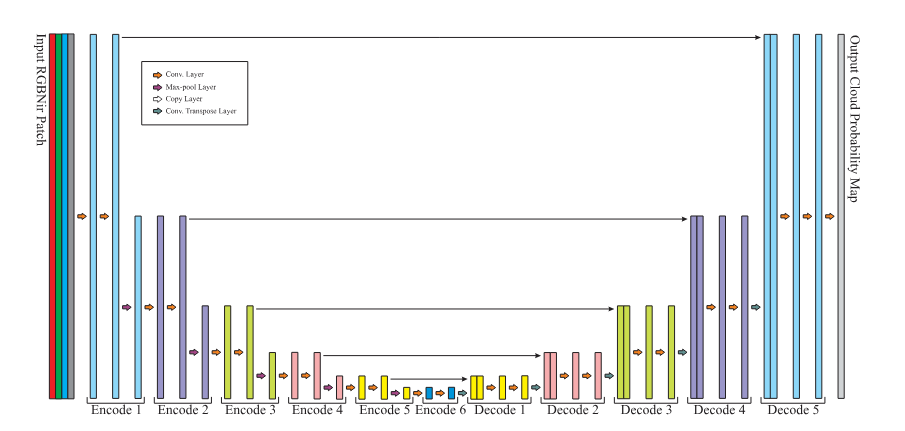
\includegraphics[width=\textwidth]{files/U-Net_cloud_detection.png}
  \caption{U-Net architecture adapted for cloud detection as used by Mohajerani et al.~\cite{mohajerani2019cloudnet}.}
  \label{fig:unet-architecture}
\end{figure}


A key innovation in U-Net is the use of residual (skip) connections \cite{he2015deepresiduallearningimage}, which dierectly link feature maps from the encoder to corresponding layers in the decoder with the same spatial size. These connections preserve fine-grained spatial details and significantly enhance segmentation quality. Moreover, they mitigate the vanishing gradient problem, facilitating the training of deeper networks and improving convergence.

\subsection{Google Coral Dev Board Mini and Edge TPU}

Running machine learning inference on embedded systems is referred to as edge inference. The Coral dev Board Mini, developed by Google, is a compact single-board computer designed for such edge AI applications. It features quad-core MediaTek 8167s System-on-a-Chip (SoC) on the Armv8-A architecture, along with a dedicated Edge TPU – a hardware accelerator optimized for executing TensorFlow Lite models using 8-bit integer operations.

The Edge TPU delivers up to 4 trillion operations per second (TOPS) of performance while consuming only around 2 watts of power, making it ideal for use in resource-constrained environments such as satellites, where energy efficiency and reliability are crucial.

To deploy a model on Edge TPU, it must meet the following requirements:
\begin{itemize}
    \item Tensor parameters quantized
    \item Tensor sizes are constant at compile-time
    \item Model parameters (such as bias tensors) are constant at compile-time
    \item Tensors are either 1-, 2-, or 3-dimensional. If a tensor has more than 3 dimensions, then only the 3 innermost dimensions may have a size greater than 1.
    \item The model uses only the operations supported by the Edge TPU (see table 1 below). \todo{CROP the table to only relevant commands and paste it}
\end{itemize}

These requirements directly affect model architecture, training strategy, and tooling. For instance, certain operations unsopported by Edge TPU must be avoided, and quantization aware training or post-training quantization must be considered early in the development process.

The following image from Coral documentation summarizes the model conversion and deployment workflow.

\begin{figure}[H]
  \centering
  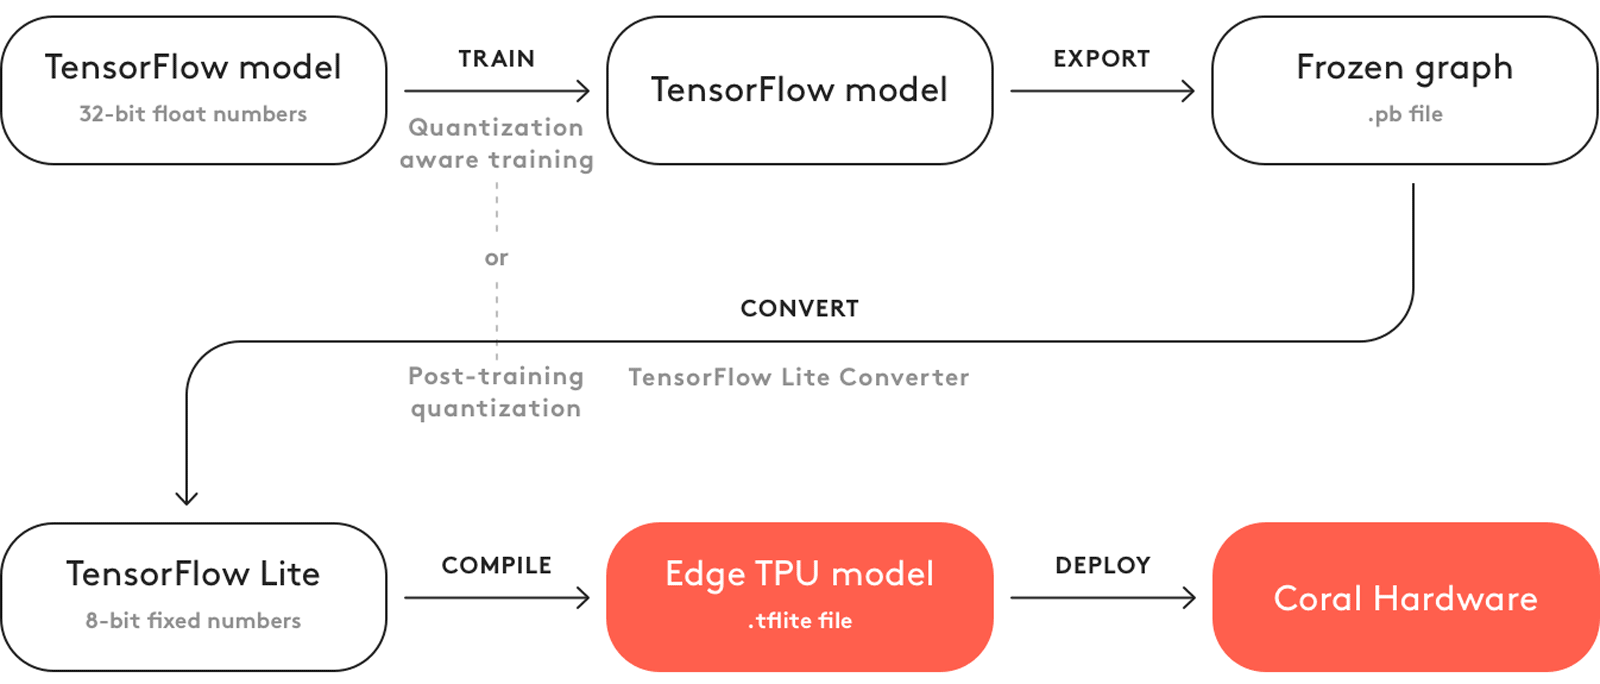
\includegraphics[width=\textwidth]{files/Edge_TPU_quantization.png}
  \caption{The basic workflow to create a model for the Edge TPU}
  \label{fig:quantization-chart}
\end{figure}

\subsection{38-Cloud Landsat 8 dataset}

Landsat 8 is an Earth observation satellite launched on February 11, 2013, providing high-resolution multispectral imagery, including visible, near infrared (NIR), and thermal infrared bands \cite{landsat8}. For cloud segmentation tasks, the red, green, blue (RGB) and NIR channels are particularly valueable due to their ability to capture both visual and athmospheric information.

This thesis utilizes a dataset consisting of 38 annotated satellite images from the Landsat 8 mission, commonly referred to as the 38-Cloud dataset \cite{38cloud}. The dataset has been introduced and adapted in the following scientific publications \cite{CloudNet2019}, \cite{CloudDet2018}. Each image contains four spectral channels (RGB and NIR), along with a manually annotated dround truth mask that labels cloud pixels at the pixel level.

The dataset is divided into a training set containing 18 scenes and a test set with the remaining 20 scenes.

}